% Created 2019-08-12 Mon 20:07
% Intended LaTeX compiler: pdflatex
\documentclass[11pt]{article}
\usepackage[utf8]{inputenc}
\usepackage[T1]{fontenc}
\usepackage{graphicx}
\usepackage{grffile}
\usepackage{longtable}
\usepackage{wrapfig}
\usepackage{rotating}
\usepackage[normalem]{ulem}
\usepackage{amsmath}
\usepackage{textcomp}
\usepackage{amssymb}
\usepackage{capt-of}
\usepackage{hyperref}
\usepackage[dvipsnames]{xcolor}
\usepackage{listings}
\usepackage{fullpage}
\hypersetup{colorlinks, citecolor=blue}
\author{Paul Bartholomew}
\date{\today}
\title{WENO Implementation in Xcompact3D}
\hypersetup{
 pdfauthor={Paul Bartholomew},
 pdftitle={WENO Implementation in Xcompact3D},
 pdfkeywords={},
 pdfsubject={},
 pdfcreator={Emacs 25.2.2 (Org mode 9.2.3)}, 
 pdflang={English}}
\begin{document}

\maketitle
\begin{abstract}
This document presents the implementation of the \texttt{weno} module for \texttt{Xcompact3D}.
It is developed as a literate program using \texttt{emacs} \texttt{org} mode.
The module itself is standalone and this is used to test it by making use of \texttt{f2py}, allowing test
cases to be quickly setup and run.
\end{abstract}
\setcounter{tocdepth}{2}
\tableofcontents

\section{Introduction}
\label{sec:org7581e9f}

In a free surface flow, the fluid properties are discontinuous at the interface between the two
fluids.
Numerically this is handled by using a smoothed step function of the form
\begin{equation}
  \rho \left( \phi \right) =
  \begin{cases}
    \rho_1 & \phi > \alpha \\ 
    \rho_2 & \phi < -\alpha \\
    \frac{\rho_1 + \rho_2}{2} + \frac{\rho_1 - \rho_2}{2} \sin\left( \frac{\pi\phi}{2\alpha} \right)
    & \mbox{otherwise}
  \end{cases} \ ,
\end{equation}
where \(\phi\) is an indicator function which is positive in fluid 1 and negative in fluid 2, its zero
contour being the interface, and \(\alpha\)>0 is a numerical interface thickness.
The indicator function is transported by the hyperbolic equation
\begin{equation}
  \frac{\partial\phi}{\partial t} + \boldsymbol{u}\cdot\boldsymbol{\nabla}\phi = 0 \ ,
\end{equation}
which when discretised requires an upwind-biased scheme to prevent oscillations in the solution.
To maintain high order away from discontinuities a \texttt{WENO} type scheme is used.

\subsection{Fifth-order WENO}
\label{sec:org905dba2}

A fifth-order \texttt{WENO} scheme (used by \cite{McSherry2017}) is given by \cite{Croce2004} as
\begin{equation}
  \left. \frac{\partial \phi}{\partial x} \right|_i =
  \begin{cases}
    \left. \frac{\partial \phi}{\partial x} \right|^-_i & u_i > 0 \\
    \left. \frac{\partial \phi}{\partial x} \right|^+_i & u_i < 0 \\
    0 & \mbox{otherwise}
  \end{cases} \ ,
\end{equation}
where superscripts + and - indicate upwind biased stencils.
These biased stencils are the weighted sum of several stencils defined around point \(i\), see
\cite{Jiang1996}, given as
\begin{equation}
  \label{eq:wenograd}
  \left. \frac{\partial \phi}{\partial x} \right|^{\pm}_i = \omega^{\pm}_1 \left(
    \frac{q^{\pm}_1}{3} - \frac{7 q^{\pm}_2}{6} + \frac{11 q^{\pm}_3}{6} \right) +
  \omega^{\pm}_2 \left( -\frac{q^{\pm}_2}{6} + \frac{5 q^{\pm}_3}{6} + \frac{q^{\pm}_4}{3} \right) +
  \omega^{\pm}_3 \left( \frac{q^{\pm}_3}{3} + \frac{5 q^{\pm}_4}{6} - \frac{q^{\pm}_5}{6} \right) \ .
\end{equation}
The fluxes in~\eqref{eq:wenograd} are given as
\begin{align}
  \begin{split}
    q^-_1 = \frac{\phi_{i - 2} - \phi_{i - 3}}{\Delta x},\ q^-_2 = \frac{\phi_{i - 1} - \phi_{i -
        2}}{\Delta x},\ q^-_3 = \frac{\phi_i - \phi_{i - 1}}{\Delta x} , \\
    q^-_4 = \frac{\phi_{i+1} - \phi_i}{\Delta x},\ q^-_5 = \frac{\phi_{i+2} - \phi_{i+1}}{\Delta x},
  \end{split} \label{eq:q-} \\
  \intertext{and}
  \begin{split}
    q^+_1 = \frac{\phi_{i+3} - \phi_{i+2}}{\Delta x},\ q^+_2 = \frac{\phi_{i+2} - \phi_{i+1}}{\Delta
      x},\ q^+_3 = \frac{\phi_{i+1} - \phi_i}{\Delta x}, \\
    q^+_4 = \frac{\phi_i - \phi_{i - 1}}{\Delta x},\ q^+_5 = \frac{\phi_{i - 1} - \phi_{i -
        2}}{\Delta x}.
  \end{split} \label{eq:q+}
\end{align}
The weights, defined such that \(\sum_{k}\omega_{k}=1\), are defined as
\begin{align}
  \omega^{\pm}_1 = \frac{\alpha^{\pm}_1}{\alpha^{\pm}_1 + \alpha^{\pm}_2 + \alpha^{\pm}_3},\
  \omega^{\pm}_2 = \frac{\alpha^{\pm}_2}{\alpha^{\pm}_1 + \alpha^{\pm}_2 + \alpha^{\pm}_3},\
  \omega^{\pm}_3 = \frac{\alpha^{\pm}_3}{\alpha^{\pm}_1 + \alpha^{\pm}_2 + \alpha^{\pm}_3},\ \label{eq:weights}\\
  \intertext{where the coefficients $\alpha_k$ are given as}
  \alpha^{\pm}_1 = \frac{1}{10}\frac{1}{{\left( \varepsilon + IS^{\pm}_1 \right)}^2},\
  \alpha^{\pm}_2 = \frac{6}{10}\frac{1}{{\left( \varepsilon + IS^{\pm}_3 \right)}^2},\
  \alpha^{\pm}_3 = \frac{3}{10}\frac{1}{{\left( \varepsilon + IS^{\pm}_3 \right)}^2}\ . \label{eq:weight-coeffs}
\end{align}
In~\eqref{eq:weight-coeffs} \(\varepsilon>0\) is a regularisation parameter (suggested \(\varepsilon=10^{-6}\)
\cite{Jiang1996,Croce2004}) and \(IS^{\pm}\) are the \texttt{WENO} smoothness indicators given as \cite{Jiang1996}
\begin{equation}
  \label{eq:smoothness-indicators}
  \begin{split}
    IS^{\pm}_1 &= \frac{13}{12} {\left( \phi_1 - 2\phi_2 + \phi_3 \right)}^2 + \frac{1}{4}
    {\left( \phi_1 - 4\phi_2 + 3\phi_3 \right)}^2\, \\
    IS^{\pm}_2 &= \frac{13}{12} {\left( \phi_2 - 2\phi_3 + \phi_4 \right)}^2 + \frac{1}{4}
    {\left( \phi_2 - \phi_4 \right)}^2\, \\
    IS^{\pm}_3 &= \frac{13}{12} {\left( \phi_3 - 2\phi_4 + \phi_5 \right)}^2 + \frac{1}{4}
    {\left( 3\phi_3 - 4\phi_4 + \phi_5 \right)}^2\ , \\
  \end{split}
\end{equation}
which ensure that each sub-stencil is given approximately equal weighting in smooth regions,
resulting in a high order scheme, whilst in the vicinity of a discontinuity the stencil(s)
containing the discontinuity are given a weighting of zero.
Near boundaries where there are not enough points, a third-order \texttt{ENO} scheme is used \cite{Croce2004}.

\section{Implementation}
\label{sec:org7a92d30}

In this section we define the \texttt{weno} module to be exported to the file \texttt{weno.f90}.

\subsection{The \texttt{weno} module}
\label{sec:orga92f4b1}

The \texttt{weno5} subroutine is defined in and exported by the \texttt{weno} module in the file \texttt{weno.f90}
(listing~\ref{orgac8f7b0}).

\lstset{basicstyle=\ttfamily\footnotesize,keywordstyle=\color{blue}\bfseries,commentstyle=\color{red},stringstyle=\color{purple},frame=single,showstringspaces=false,language=[90]Fortran,label=orgac8f7b0,caption={The \texttt{weno} module.},captionpos=b,numbers=none}
\begin{lstlisting}
module weno

  implicit none

  private
  public :: weno5

contains

  <<src:weno5.f90>>

endmodule weno
\end{lstlisting}

\subsection{The \texttt{weno5} subroutine}
\label{sec:org7acb819}

The \texttt{weno5} subroutine takes as input 3D arrays of the variable whose gradient is to be evaluated
and the advecting velocity field, returning a 3D array of the gradient.
Additional input variables are the boundary conditions, array sizes and the mesh spacing.

\lstset{basicstyle=\ttfamily\footnotesize,keywordstyle=\color{blue}\bfseries,commentstyle=\color{red},stringstyle=\color{purple},frame=single,showstringspaces=false,language=[90]Fortran,label=orgef1b7b1,caption={\texttt{WENO} subroutine definition.},captionpos=b,numbers=none}
\begin{lstlisting}
subroutine weno5(gradphi, phi, advvel, &
     axis, bc0, bcn, &
     isize, jsize, ksize, &
     dx, dy, dz)

  implicit none

  <<src:weno5-declarations.f90>>

  <<src:weno5-setup.f90>>

  do k = kstart, kend
     do j = jstart, jend
	!! Note, if axis==2 and y is stretched, need to set deltax here
	do i = istart, iend
	   <<src:sign.f90>>
	   <<src:calcq.f90>>
	   <<src:calcsmooth.f90>>
	   <<src:calcweights.f90>>
	   <<src:calcgrad.f90>>
	enddo

	<<src:bcx.f90>>
     enddo

     <<src:bcy.f90>>
  enddo

  <<src:bcz.f90>>

endsubroutine weno5
\end{lstlisting}

Following the variable declarations and some setup code (given in
listings~\ref{org2e2a3f9} and~\ref{orgbbc7c02} respectively), the heart of the \texttt{weno5}
subroutine is the loop over the internal (\emph{i.e.} non-boundary) nodes of the 3D arrays where the
gradient is evaluated using code developed in the subsequent subsections.
The implementation of boundary conditions is rather more involved due to the need to handle the
three nodes closest to the boundary and is given in~\S\ref{sec:orga10c0cf}.

\lstset{basicstyle=\ttfamily\footnotesize,keywordstyle=\color{blue}\bfseries,commentstyle=\color{red},stringstyle=\color{purple},frame=single,showstringspaces=false,language=[90]Fortran,label=orgbbc7c02,caption={Setup code for \texttt{weno5} subroutine.},captionpos=b,numbers=none}
\begin{lstlisting}
!! Defaults
istart = 1
iend = isize
jstart = 1
jend = jsize
kstart = 1
kend = ksize

istep = 0
jstep = 0
kstep = 0

if (axis==1) then
   deltax = dx

   istart = 4
   iend = isize - 3
   istep = 1
elseif (axis==2) then
   deltax = dy

   jstart = 4
   jend = jsize - 3
   jstep = 1
elseif (axis==3) then
   deltax = dz

   kstart = 4
   kend = ksize - 3
   kstep = 1
else
   print *, "ERROR: Invalid axis passed to WENO5"
   stop
endif
\end{lstlisting}

\lstset{basicstyle=\ttfamily\footnotesize,keywordstyle=\color{blue}\bfseries,commentstyle=\color{red},stringstyle=\color{purple},frame=single,showstringspaces=false,language=[90]Fortran,label=org2e2a3f9,caption={Variable declarations for \texttt{weno5} subroutine.},captionpos=b,numbers=none}
\begin{lstlisting}
integer, intent(in) :: axis
integer, intent(in) :: bc0, bcn
integer, intent(in) :: isize, jsize, ksize
real(kind=8), intent(in) :: dx, dy, dz
real(kind=8), dimension(isize, jsize, ksize), intent(in) :: phi
real(kind=8), dimension(isize, jsize, ksize), intent(in) :: advvel

real(kind=8), dimension(isize, jsize, ksize), intent(inout) :: gradphi

integer :: i, j, k
integer :: istep, jstep, kstep
integer :: istart, jstart, kstart, iend, jend, kend
integer :: im1, im2, im3, ip1, ip2
integer :: jm1, jm2, jm3, jp1, jp2
integer :: km1, km2, km3, kp1, kp2
real(kind=8), parameter :: e = 1.0d-16
real(kind=8), parameter :: zero = 0.d0, &
     one = 1.d0, &
     two = 2.d0, &
     three = 3.d0, &
     four = 4.d0, &
     five = 5.d0, &
     six = 6.d0, &
     seven = 7.d0, &
     ten = 10.d0, &
     eleven = 11.d0, &
     twelve = 12.d0, &
     thirteen = 13.d0

real(kind=8) :: q1, q2, q3, q4, q5
real(kind=8) :: a1, a2, a3
real(kind=8) :: w1, w2, w3
real(kind=8) :: is1, is2, is3
real(kind=8) :: dsign
real(kind=8) :: deltax
\end{lstlisting}

\subsection{Gradient evaluation}
\label{sec:orgafb6472}

At each point, the gradient evaluation follows directly from the definition in~\eqref{eq:wenograd},
given in listing~\ref{orge0155cb}.

\lstset{basicstyle=\ttfamily\footnotesize,keywordstyle=\color{blue}\bfseries,commentstyle=\color{red},stringstyle=\color{purple},frame=single,showstringspaces=false,language=[90]Fortran,label=orge0155cb,caption={Evaluation of \(\partial \phi\)/\(\partial\)x using fifth-order \texttt{WENO} scheme.},captionpos=b,numbers=none}
\begin{lstlisting}
gradphi(i, j, k) = w1 * (two * q1 - seven * q2 + eleven * q3) &
     + w2 * (-q2 + five * q3 + two * q4) &
     + w3 * (two * q3 + five * q4 - q5)
gradphi(i, j, k) = gradphi(i, j, k) / six
\end{lstlisting}

\subsection{Stencil computation}
\label{sec:orgd3cc3f9}

The stencils \(q^{\pm}_k\) are computed in listing~\ref{orgea3a4f0}.

\lstset{basicstyle=\ttfamily\footnotesize,keywordstyle=\color{blue}\bfseries,commentstyle=\color{red},stringstyle=\color{purple},frame=single,showstringspaces=false,language=[90]Fortran,label=orgea3a4f0,caption={Stencil evaluation for fifth-order \texttt{WENO} scheme.},captionpos=b,numbers=none}
\begin{lstlisting}
q1 = dsign * (phi(im2, jm2, km2) - phi(im3, jm3, km3)) / deltax
q2 = dsign * (phi(im1, jm1, km1) - phi(im2, jm2, km2)) / deltax
q3 = dsign * (phi(i, j, k) - phi(im1, jm1, km1)) / deltax
q4 = dsign * (phi(ip1, jp1, kp1) - phi(i, j, k)) / deltax
q5 = dsign * (phi(ip2, jp2, kp2) - phi(ip1, jp1, kp1)) / deltax
\end{lstlisting}

By exploiting the symmetry of~\eqref{eq:q-}
and~\eqref{eq:q+} the stencils can be computed in the same way by setting the array indices and sign
of the equation according to the flow direction and coordinate axis.
This is achieved by \texttt{dsign} indicating the flow direction and index offsets computed in
listing~\ref{org8865c6e}.

\lstset{basicstyle=\ttfamily\footnotesize,keywordstyle=\color{blue}\bfseries,commentstyle=\color{red},stringstyle=\color{purple},frame=single,showstringspaces=false,language=[90]Fortran,label=org8865c6e,caption={Stencil sign and index offsets.},captionpos=b,numbers=none}
\begin{lstlisting}
if (advvel(i, j, k) > zero) then
   dsign = one

   istep = istep
   jstep = jstep
   kstep = kstep
elseif (advvel(i, j, k) < zero) then
   dsign = -one

   istep = -istep
   jstep = -jstep
   kstep = -kstep
else
   gradphi(i, j, k) = zero
   cycle
endif

im1 = i - 1 * istep
im2 = i - 2 * istep
im3 = i - 3 * istep
ip1 = i + 1 * istep
ip2 = i + 2 * istep

jm1 = j - 1 * jstep
jm2 = j - 2 * jstep
jm3 = j - 3 * jstep
jp1 = j + 1 * jstep
jp2 = j + 2 * jstep

km1 = k - 1 * kstep
km2 = k - 2 * kstep
km3 = k - 3 * kstep
kp1 = k + 1 * kstep
kp2 = k + 2 * kstep
\end{lstlisting}

\subsection{Weight evaluation}
\label{sec:org5b8a607}

To complete the computation of the gradients the stencil weights are calculated in
listing~\ref{orgf5878a4} with the smoothness indicators defined in listing~\ref{orge64be70}
according to~\eqref{eq:weight-coeffs},~\eqref{eq:weights} and~\eqref{eq:smoothness-indicators}
respectively.

\lstset{basicstyle=\ttfamily\footnotesize,keywordstyle=\color{blue}\bfseries,commentstyle=\color{red},stringstyle=\color{purple},frame=single,showstringspaces=false,language=[90]Fortran,label=orgf5878a4,caption={Weight calculation for fifth-order \texttt{WENO} scheme.},captionpos=b,numbers=none}
\begin{lstlisting}
a1 = one / (e + is1)**2 / ten
a2 = six / (e + is2)**2 / ten
a3 = three / (e + is3)**2 / ten

w1 = a1 / (a1 + a2 + a3)
w2 = a2 / (a1 + a2 + a3)
w3 = a3 / (a1 + a2 + a3)
\end{lstlisting}

\lstset{basicstyle=\ttfamily\footnotesize,keywordstyle=\color{blue}\bfseries,commentstyle=\color{red},stringstyle=\color{purple},frame=single,showstringspaces=false,language=[90]Fortran,label=orge64be70,caption={Smoothness indicators for fifth-order \texttt{WENO} scheme.},captionpos=b,numbers=none}
\begin{lstlisting}
is1 = (thirteen / twelve) * (phi(im2,jm2,km2) - two * phi(im1,jm1,km1) + phi(i,j,k))**2 &
     + (phi(im2,jm2,km2) - four * phi(im1,jm1,km1) + three * phi(i,j,k))**2 / four
is2 = (thirteen / twelve) * (phi(im1,jm1,km1) - two * phi(i,j,k) + phi(ip1,jp1,kp1))**2 &
     + (phi(im1,jm1,km1) - phi(ip1,jp1,kp1))**2 / four
is3 = (thirteen / twelve) * (phi(i,j,k) - two * phi(ip1,jp1,kp1) + phi(ip2,jp2,kp2))**2 &
     + (three * phi(i,j,k) - four * phi(ip1,jp1,kp1) + phi(ip2,jp2,kp2))**2 / four
\end{lstlisting}

\section{Testing}
\label{sec:orgaf5e925}

To avoid the need to define and run a full-fledged simulation to test the implementation, \texttt{f2py} will
is used to build a python module from \texttt{weno.f90} using the \texttt{Makefile} defined in listing~\ref{org2a74e9f}.
Typing \texttt{make} will build the module (requires \texttt{numpy} and a \texttt{Fortran} compiler).

\lstset{basicstyle=\ttfamily\footnotesize,keywordstyle=\color{blue}\bfseries,commentstyle=\color{red},stringstyle=\color{purple},frame=single,showstringspaces=false,language=make,label=org2a74e9f,caption={Makefile to build \texttt{weno} python module},captionpos=b,numbers=none}
\begin{lstlisting}
all:
  python -m numpy.f2py -c weno.f90 -m weno
\end{lstlisting}

\subsection{Testing derivative evaluation}
\label{sec:org563f577}

To test the code we first look at computing the derivative of \(f\left(x\right)=\sin\left(x\right)\),
\(f'\left(x\right)=\cos\left(x\right)\) in the \(x\), \(y\) and \(z\) directions.

\lstset{basicstyle=\ttfamily\footnotesize,keywordstyle=\color{blue}\bfseries,commentstyle=\color{red},stringstyle=\color{purple},frame=single,showstringspaces=false,language=Python,label=org5192dea,caption={Computing derivative of \(\sin\left(x\right)\) in \(x\), \(y\) and \(z\) directions using \texttt{weno5}.},captionpos=b,numbers=none}
\begin{lstlisting}
<<src:import.py>>

<<src:dom-f-def.py>>

# Test x
<<src:xsetup.py>>
<<src:xinit.py>>
<<src:gradx.py>>
<<src:plotx.py>>

# Test y
<<src:ysetup.py>>
<<src:yinit.py>>
<<src:grady.py>>
<<src:ploty.py>>

# Test z
<<src:zsetup.py>>
<<src:zinit.py>>
<<src:gradz.py>>
<<src:plotz.py>>

# Test with discontinuity
<<src:shift.py>>
<<src:test-discontinuous.py>>
\end{lstlisting}

The code requires importing the \texttt{math}, \texttt{numpy} and \texttt{matplotlib} modules and of course the \texttt{weno5} function
\lstset{basicstyle=\ttfamily\footnotesize,keywordstyle=\color{blue}\bfseries,commentstyle=\color{red},stringstyle=\color{purple},frame=single,showstringspaces=false,language=Python,label=org42f244b,caption={Imports to test the \texttt{weno5} function in python},captionpos=b,numbers=none}
\begin{lstlisting}
import math
import numpy as np
import matplotlib.pyplot as plt

import weno
weno5 = weno.weno.weno5
\end{lstlisting}

The domain, function and analytical gradient is defined as:
\lstset{basicstyle=\ttfamily\footnotesize,keywordstyle=\color{blue}\bfseries,commentstyle=\color{red},stringstyle=\color{purple},frame=single,showstringspaces=false,language=Python,label=org11a2e54,caption={Domain and function definition},captionpos=b,numbers=none}
\begin{lstlisting}
N = 100
L = 2 * math.pi

dx = L / (N - 1.0)
x = []
f = []
fp = []
for i in range(N):
  x.append(i * dx)
  f.append(math.sin(x[i]))
  fp.append(math.cos(x[i]))
\end{lstlisting}

Using the \(x\) axis as an example, we first create arrays to hold the advecting velocity, \(\phi\) and the
gradient
\lstset{basicstyle=\ttfamily\footnotesize,keywordstyle=\color{blue}\bfseries,commentstyle=\color{red},stringstyle=\color{purple},frame=single,showstringspaces=false,language=Python,label=org36ba605,caption={Code to setup the arrays for computing the gradient in \(x\)},captionpos=b,numbers=none}
\begin{lstlisting}
u = np.zeros((N, 1, 1), dtype=np.float64, order="F")
phi = np.zeros((N, 1, 1), dtype=np.float64, order="F")
gradphi = np.zeros((N, 1, 1), dtype=np.float64, order="F")
\end{lstlisting}
and set their values to 1, the \(f\left(x\right)\) and 0 respectively
\lstset{basicstyle=\ttfamily\footnotesize,keywordstyle=\color{blue}\bfseries,commentstyle=\color{red},stringstyle=\color{purple},frame=single,showstringspaces=false,language=Python,label=org9d2866a,caption={Setting the input and zeroing the output for gradient computation},captionpos=b,numbers=none}
\begin{lstlisting}
for i in range(N):
  for j in range(1):
    for k in range(1):
      u[i][j][k] = 1.0
      phi[i][j][k] = f[i]
      gradphi[i][j][k] = 0.0
\end{lstlisting}
We are now ready to compute the gradient by calling \texttt{weno5}
\lstset{basicstyle=\ttfamily\footnotesize,keywordstyle=\color{blue}\bfseries,commentstyle=\color{red},stringstyle=\color{purple},frame=single,showstringspaces=false,language=Python,label=org2519b9b,caption={Computing the gradient using \texttt{weno5}},captionpos=b,numbers=none}
\begin{lstlisting}
weno5(gradphi, phi, u, 1, 2, 2, dx, dx, dx)
\end{lstlisting}
Finally the computed gradient is plotted against the analytical solution, shown in
\emph{figs}.~\ref{fig:orgc21fdc6},~\ref{fig:org4c112b5} and~\ref{fig:org7947a10} for the \(x\), \(y\) and \(z\)
axes respectively.
\lstset{basicstyle=\ttfamily\footnotesize,keywordstyle=\color{blue}\bfseries,commentstyle=\color{red},stringstyle=\color{purple},frame=single,showstringspaces=false,language=Python,label=orgf245894,caption={Plotting the computed and analytical gradients},captionpos=b,numbers=none}
\begin{lstlisting}
fpc = np.zeros(N)
for i in range(N):
  fpc[i] = gradphi[i][0][0]
plt.plot(x, fpc, marker="o")
plt.plot(x, fp)
plt.title("Test x-derivative (smooth)")
plt.savefig("weno-smoothx.eps", bbox_inches="tight")
plt.close()
\end{lstlisting}
\begin{figure}[htbp]
\centering
\includegraphics[width=0.5\textwidth]{./weno-smoothx.eps}
\caption{\label{fig:orgc21fdc6}
\texttt{WENO5} derivative of \(f\left(x\right)=\sin\left(x\right)\) compared with \(f'\left(x\right)=\cos\left(x\right)\).}
\end{figure}

\begin{figure}[htbp]
\centering
\includegraphics[width=0.5\textwidth]{./weno-smoothy.eps}
\caption{\label{fig:org4c112b5}
\texttt{WENO5} derivative of \(f\left(y\right)=\sin\left(y\right)\) compared with \(f'\left(y\right)=\cos\left(y\right)\).}
\end{figure}

\begin{figure}[htbp]
\centering
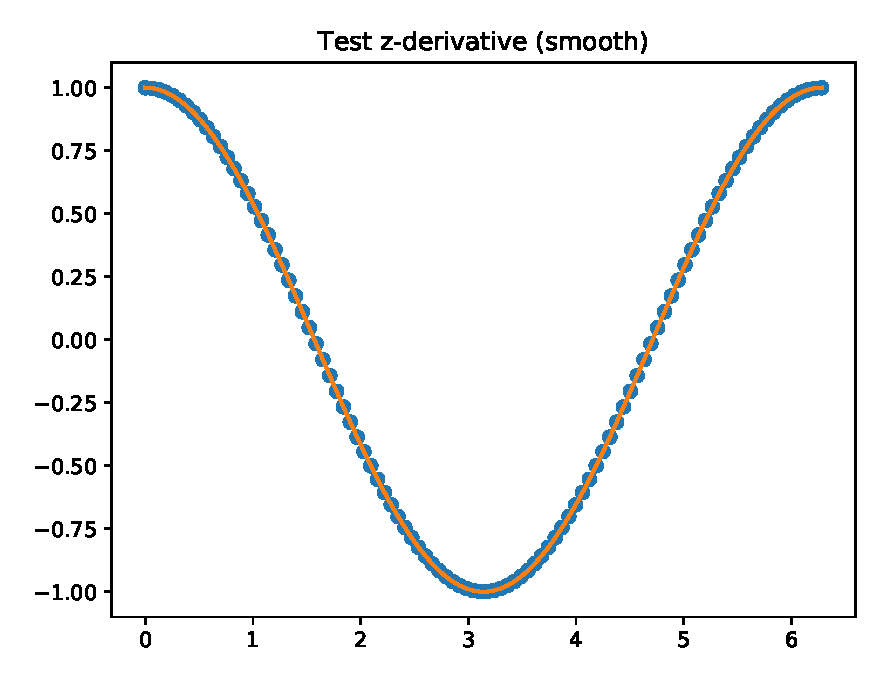
\includegraphics[width=0.5\textwidth]{./weno-smoothz.eps}
\caption{\label{fig:org7947a10}
\texttt{WENO5} derivative of \(f\left(z\right)=\sin\left(z\right)\) compared with \(f'\left(z\right)=\cos\left(z\right)\).}
\end{figure}

\pagebreak

A more challenging test is the ability to compute derivatives with a discontinuity, we achieve this
by shifting the field by 1 over the last half of the domain:
\lstset{basicstyle=\ttfamily\footnotesize,keywordstyle=\color{blue}\bfseries,commentstyle=\color{red},stringstyle=\color{purple},frame=single,showstringspaces=false,language=Python,label=orgd82565c,caption={Code to shift field},captionpos=b,numbers=none}
\begin{lstlisting}
for i in range(N/2, N):
  f[i] += 1
\end{lstlisting}
and we test this over the x axis
\lstset{basicstyle=\ttfamily\footnotesize,keywordstyle=\color{blue}\bfseries,commentstyle=\color{red},stringstyle=\color{purple},frame=single,showstringspaces=false,language=Python,label=orgb0b5e18,caption={Compute and plot derivative of discontinuous field},captionpos=b,numbers=none}
\begin{lstlisting}
# Test x
u = np.zeros((N, 1, 1), dtype=np.float64, order="F")
phi = np.zeros((N, 1, 1), dtype=np.float64, order="F")
gradphi = np.zeros((N, 1, 1), dtype=np.float64, order="F")
for i in range(N):
  for j in range(1):
    for k in range(1):
      u[i][j][k] = 1.0
      phi[i][j][k] = f[i]
      gradphi[i][j][k] = 0.0

weno5(gradphi, phi, u, 1, 2, 2, dx, dx, dx)

fpc = np.zeros(N)
for i in range(N):
  fpc[i] = gradphi[i][0][0]
plt.plot(x, fpc, marker="o")
plt.title("Test x-derivative (discontinuous)")
plt.savefig("weno-discontinuousx.eps")
plt.close()
\end{lstlisting}
resulting in the approximate derivative shown in \emph{fig.}~\ref{fig:org9d0a42c} (note that either
side of the discontinuity the derivative approximates \(f'\left(x\right)=\cos\left(x\right)\) well).

\begin{figure}[htbp]
\centering
\includegraphics[width=0.5\textwidth]{./weno-discontinuousx.eps}
\caption{\label{fig:org9d0a42c}
\texttt{WENO5} derivative of \(f\left(x\right)=\sin\left(x\right)\) with discontinuity at \(x=\pi\).}
\end{figure}

\pagebreak

\subsection{Testing an advection equation}
\label{sec:orga77be55}

As a more realistic test, consider the advection equation
\begin{equation}
  \frac{\partial\phi}{\partial t} + \boldsymbol{u}\cdot\boldsymbol{\nabla}\phi = 0
\end{equation}
which we will solve in one-dimension, using explicit time advancement and a prescribed velocity
field.
We will use the explicit integrator provided by \texttt{scipy} to integrate the function.
The code to calculate the right hand side is given in listing~\ref{org512e78c}.

\lstset{basicstyle=\ttfamily\footnotesize,keywordstyle=\color{blue}\bfseries,commentstyle=\color{red},stringstyle=\color{purple},frame=single,showstringspaces=false,language=Python,label=org512e78c,caption={Compute the right hand side of advection equation},captionpos=b,numbers=none}
\begin{lstlisting}
def calc_rhs(t, y, f_args):
    u = f_args[0]  # The velocity field
    dx = f_args[1] # The grid spacing
    n = len(y)

    y3d = np.array(y).reshape((n, 1, 1), order="F")
    u3d = u * np.ones(n).reshape((n, 1, 1), order="F")
    dydx = np.zeros((n, 1, 1), order="F")

    weno5(dydx, y3d, u3d, 1, 0, 0, dx, dx, dx)

    return -u*dydx.reshape(n)

\end{lstlisting}

As an initial field we will consider the function used by \cite{Jiang1996}
\begin{equation}
  \phi \left( x, 0 \right) =
  \begin{cases}
    \frac{1}{6} \left( g \left(x, \beta, z - \delta \right) + g\left(x, \beta, z + \delta \right) +
      4g \left(x, \beta, z \right), \right) & -0.8\leq x \leq-0.6 \\
    1 & -0.4 \leq x \leq -0.2 \\
    1 - \left|10\left(x-0.1\right)\right| & 0 \leq x \leq 0.2\\
    \frac{1}{6} \left( f \left(x, \alpha, a - \delta \right) + f\left(x, \alpha, a + \delta \right) +
      4f \left(x, \alpha, a \right), \right) & 0.4\leq x \leq 0.6 \\
    0 & \mbox{otherwise}
  \end{cases}
\end{equation}
where \(g\left(x,\beta,z\right)=e^{-\beta\left(x-z\right)^2}\) and
\(f\left(x,\alpha,a\right)=\sqrt(max\left(1 - \alpha^{2}\left(x-a\right)^{2}, 0\right)\) with the associated
initialisation code in listing~\ref{org8d0ae6d}

\lstset{basicstyle=\ttfamily\footnotesize,keywordstyle=\color{blue}\bfseries,commentstyle=\color{red},stringstyle=\color{purple},frame=single,showstringspaces=false,language=Python,label=org8d0ae6d,caption={Initialisation function for advection test},captionpos=b,numbers=none}
\begin{lstlisting}
def init_jiang(x):

    phi = []
    n = len(x)

    a = 0.5
    z = -0.7
    d = 0.005
    alpha = 10.0
    beta = log10(2.0) / (36 * d**2)

    for i in range(n):
	if (-0.8 <= x[i]) and (x[i] <= -0.6):
	    phi.append(g(x[i], beta, z - d) + g(x[i], beta, z + d) + 4 * g(x[i], beta, z))
	    phi[-1] /= 6.0
	elif (-0.4 <= x[i]) and (x[i] <= -0.2):
	    phi.append(1)
	elif (0 <= x[i]) and (x[i] <= 0.2):
	    phi.append(1 - abs(10 * (x[i] - 0.1)))
	elif (0.4 <= x[i]) and (x[i] <= 0.6):
	    phi.append(f(x[i], alpha, a - d) + f(x[i], alpha, a + d) + 4 * f(x[i], alpha, a))
	    phi[-1] /= 6.0
	else:
	    phi.append(0)

    return phi

def g(x, b, z):
    return exp(-b * (x - z)**2)

def f(x, alpha, a):
    return sqrt(max(1 - (alpha**2) * (x - a)**2, 0))
\end{lstlisting}

The code to perform the integration is then
\lstset{basicstyle=\ttfamily\footnotesize,keywordstyle=\color{blue}\bfseries,commentstyle=\color{red},stringstyle=\color{purple},frame=single,showstringspaces=false,language=Python,label= ,caption= ,captionpos=b,numbers=none}
\begin{lstlisting}
from math import sin, pi, log, log10, sqrt, exp
import numpy as np
from scipy.integrate import ode
import matplotlib.pyplot as plt
import weno
weno5 = weno.weno.weno5

<<src:jiang-init.py>>
<<src:rhs.py>>
<<src:rk3.py>>

L=2.0
U=1.0
N=200
CFL = 0.2
T=10

dx=L/float(N)
x = []
for i in range(N):
    x.append(i * dx - 1)
xl = -0.2
xr = 0.2

dt = CFL * dx / U

# r = ode(calc_rhs).set_integrator("dopri5", atol=1.0e-16, rtol=1.0e-8)
r = rk3(calc_rhs)
r.set_initial_value(init_jiang(x))
r.set_f_params((U, dx))

passed_eight = False
while r.successful() and r.t < T:
    if r.t == 0:
	plt.plot(x, r.y, color="black")
    elif (r.t >= 8) and (not passed_eight):
	plt.plot(x, r.y, ls="", marker="o", color="blue")
	passed_eight = True
    print r.t, min(r.y), max(r.y)
    r.integrate(r.t+dt)

plt.plot(x, r.y, ls="", marker="o", color="red")
plt.savefig("adv_test.eps", bbox_inches="tight")
\end{lstlisting}

To confirm the integration was working, an RK3 function was implemented according to \cite{Croce2004},
implementing the same interface as \texttt{ode} from \texttt{scipy}.

\lstset{basicstyle=\ttfamily\footnotesize,keywordstyle=\color{blue}\bfseries,commentstyle=\color{red},stringstyle=\color{purple},frame=single,showstringspaces=false,language=Python,label=org3f06378,caption={Runge-Kutta 3 implementation},captionpos=b,numbers=none}
\begin{lstlisting}
class rk3():

    def __init__(self, f, t = 0):

	self.f = f
	self.t = 0

    def set_initial_value(self, y0):

	self.y = y0

    def set_f_params(self, f_args):
	self.f_args = f_args

    def successful(self):
	return True

    def integrate(self, tnext):

	dt = tnext - self.t

	# Stage 1
	f0 = self.f(self.t, self.y, self.f_args)
	y1 = self.y + dt * f0

	# Stage 2
	f1 = self.f(self.t, y1, self.f_args)
	y2 = self.y + (dt / 4.0) * (f0 + f1)

	# Stage 3
	f2 = self.f(self.t, y2, self.f_args)
	self.y += (dt / 6.0) * (f0 + 4 * f2 + f1)

	self.t += dt
\end{lstlisting}

The result is compared with the analytical solution at \(t=8, 10\) in \emph{fig.}~\ref{fig:org963ffb9} and shows
excellent agreement compared with results in the literature \cite{Jiang1996} with the maxima and
minima well captured.

\begin{figure}[htbp]
\centering
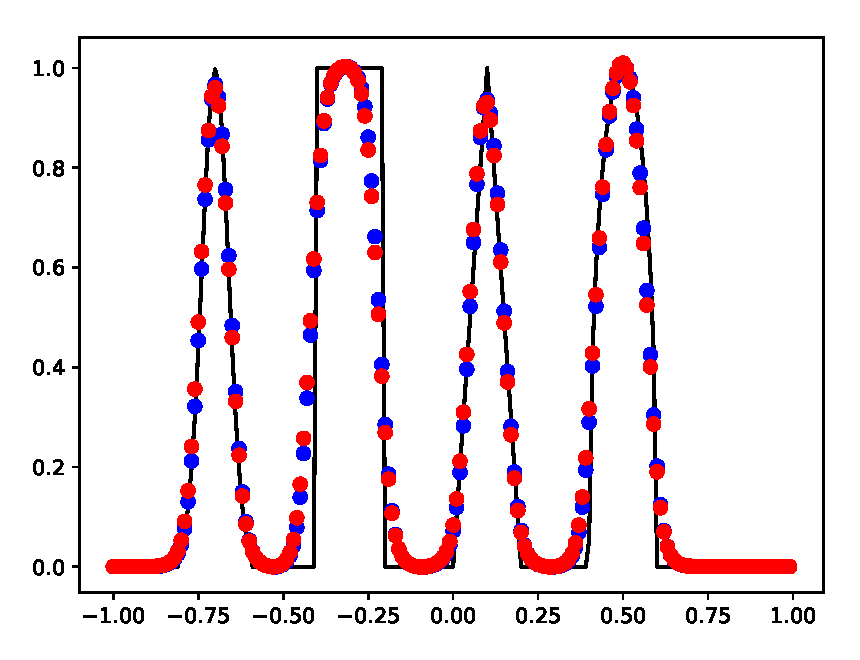
\includegraphics[width=0.5\textwidth]{./adv_test.eps}
\caption{\label{fig:org963ffb9}
Comparison of solution of advection equation with analytical solution}
\end{figure}


\section{Backmatter}
\label{sec:org8cfe36a}

\bibliography{../../../../Documents/Postdoc}
\bibliographystyle{plain}

\appendix

\section{Appendices}
\label{sec:org7175f83}

\subsection{Boundary conditions}
\label{sec:orga10c0cf}

\lstset{basicstyle=\ttfamily\footnotesize,keywordstyle=\color{blue}\bfseries,commentstyle=\color{red},stringstyle=\color{purple},frame=single,showstringspaces=false,language=[90]Fortran,label=orgb3b5c4a,caption={x-boundary conditions},captionpos=b,numbers=none}
\begin{lstlisting}
if (axis==1) then
   jm1 = j
   jm2 = j
   jm3 = j
   jp1 = j
   jp2 = j

   km1 = k
   km2 = k
   km3 = k
   kp1 = k
   kp2 = k

   if ((bc0==0).and.(bcn==0)) then
      i = 1
      if (advvel(i, j, k) == zero) then
	 gradphi(i, j, k) = zero
      else
	 if (advvel(i, j, k) > zero) then
	    dsign = one

	    im1 = isize
	    im2 = isize - 1
	    im3 = isize - 2
	    ip1 = i + 1
	    ip2 = i + 2
	 else
	    dsign = -one

	    im1 = i + 1
	    im2 = i + 2
	    im3 = i + 3
	    ip1 = isize
	    ip2 = isize - 1
	 endif
	 <<src:calcq.f90>>
	 <<src:calcsmooth.f90>>
	 <<src:calcweights.f90>>
	 <<src:calcgrad.f90>>
      endif

      i = 2
      if (advvel(i, j, k) == zero) then
	 gradphi(i, j, k) = zero
      else
	 if (advvel(i, j, k) > zero) then
	    dsign = one

	    im1 = i - 1
	    im2 = isize
	    im3 = isize - 1
	    ip1 = i + 1
	    ip2 = i + 2
	 else
	    dsign = -one

	    im1 = i + 1
	    im2 = i + 2
	    im3 = i + 3
	    ip1 = i - 1
	    ip2 = isize
	 endif
	 <<src:calcq.f90>>
	 <<src:calcsmooth.f90>>
	 <<src:calcweights.f90>>
	 <<src:calcgrad.f90>>
      endif

      i = 3
      if (advvel(i, j, k) == zero) then
	 gradphi(i, j, k) = zero
      else
	 if (advvel(i, j, k) > zero) then
	    dsign = one

	    im1 = i - 1
	    im2 = i - 2
	    im3 = isize
	    ip1 = i + 1
	    ip2 = i + 2
	 else
	    dsign = -one

	    im1 = i + 1
	    im2 = i + 2
	    im3 = i + 3
	    ip1 = i - 1
	    ip2 = i - 2
	 endif
	 <<src:calcq.f90>>
	 <<src:calcsmooth.f90>>
	 <<src:calcweights.f90>>
	 <<src:calcgrad.f90>>
      endif

      i = isize
      if (advvel(i, j, k)==zero) then
	 gradphi(i, j, k) = zero
      else
	 if (advvel(i, j, k) > zero) then
	    dsign = one

	    im1 = i - 1
	    im2 = i - 2
	    im3 = i - 3
	    ip1 = 1
	    ip2 = 2
	 else
	    dsign = -one

	    im1 = 1
	    im2 = 2
	    im3 = 3
	    ip1 = i - 1
	    ip2 = i - 2
	 endif
	 <<src:calcq.f90>>
	 <<src:calcsmooth.f90>>
	 <<src:calcweights.f90>>
	 <<src:calcgrad.f90>>
      endif

      i = isize - 1
      if (advvel(i, j, k) == zero) then
	 gradphi(i, j, k) = zero
      else
	 if (advvel(i, j, k) > zero) then
	    dsign = one

	    im1 = i - 1
	    im2 = i - 2
	    im3 = i - 3
	    ip1 = i + 1
	    ip2 = 1
	 else
	    dsign = -one

	    im1 = i + 1
	    im2 = 1
	    im3 = 2
	    ip1 = i - 1
	    ip2 = i - 2
	 endif
	 <<src:calcq.f90>>
	 <<src:calcsmooth.f90>>
	 <<src:calcweights.f90>>
	 <<src:calcgrad.f90>>
      endif

      i = isize - 2
      if (advvel(i, j, k) == zero) then
	 gradphi(i, j, k) = zero
      else
	 if (advvel(i, j, k) > zero) then
	    dsign = one

	    im1 = i - 1
	    im2 = i - 2
	    im3 = i - 3
	    ip1 = i + 1
	    ip2 = i + 2
	 else
	    dsign = -one

	    im1 = i + 1
	    im2 = i + 2
	    im3 = 1
	    ip1 = i - 1
	    ip2 = i - 2
	 endif
	 <<src:calcq.f90>>
	 <<src:calcsmooth.f90>>
	 <<src:calcweights.f90>>
	 <<src:calcgrad.f90>>
      endif
   else
      !! Use second order
      i = 1
      if (bc0==1) then ! Zero grad
	 gradphi(i, j, k) = zero
      else ! Fixed value
	 gradphi(i, j, k) = (phi(i + 1, j, k) - phi(i, j, k)) / dx
      endif
      do i = 2, 3
	 gradphi(i, j, k) = (phi(i + 1, j, k) - phi(i - 1, j, k)) / (two * dx)
      enddo

      do i = isize - 2, isize - 1
	 gradphi(i, j, k) = (phi(i + 1, j, k) - phi(i - 1, j, k)) / (two * dx)
      enddo
      i = isize
      if (bcn==1) then ! Zero grad
	 gradphi(i, j, k) = zero
      else
	 gradphi(i, j, k) = (phi(i, j, k) - phi(i - 1, j, k)) / dx
      endif
   endif
endif
\end{lstlisting}

\lstset{basicstyle=\ttfamily\footnotesize,keywordstyle=\color{blue}\bfseries,commentstyle=\color{red},stringstyle=\color{purple},frame=single,showstringspaces=false,language=[90]Fortran,label=org0aaf619,caption={y-boundary conditions},captionpos=b,numbers=none}
\begin{lstlisting}
if (axis==2) then
   km1 = k
   km2 = k
   km3 = k
   kp1 = k
   kp2 = k

   if ((bc0==0).and.(bcn==0)) then
      j = 1

      do i = 1, isize
	 im1 = i
	 im2 = i
	 im3 = i
	 ip1 = i
	 ip2 = i

	 if (advvel(i, j, k)==zero) then
	    gradphi(i, j, k) = zero
	 else
	    if (advvel(i, j, k) > zero) then
	       dsign = one

	       jm1 = jsize
	       jm2 = jsize - 1
	       jm3 = jsize - 2
	       jp1 = j + 1
	       jp2 = j + 2
	    else
	       dsign = -one

	       jm1 = j + 1
	       jm2 = j + 2
	       jm3 = j + 3
	       jp1 = jsize
	       jp2 = jsize - 1
	    endif
	    <<src:calcq.f90>>
	    <<src:calcsmooth.f90>>
	    <<src:calcweights.f90>>
	    <<src:calcgrad.f90>>
	 endif

	 j = 2
	 if (advvel(i, j, k)==zero) then
	    gradphi(i, j, k) = zero
	 else
	    if (advvel(i, j, k) > zero) then
	       dsign = one

	       jm1 = j - 1
	       jm2 = jsize
	       jm3 = jsize - 1
	       jp1 = j + 1
	       jp2 = j + 2
	    else
	       dsign = -one

	       jm1 = j + 1
	       jm2 = j + 2
	       jm3 = j + 3
	       jp1 = j - 1
	       jp2 = jsize
	    endif
	    <<src:calcq.f90>>
	    <<src:calcsmooth.f90>>
	    <<src:calcweights.f90>>
	    <<src:calcgrad.f90>>
	 endif

	 j = 3
	 if (advvel(i, j, k)==zero) then
	    gradphi(i, j, k) = zero
	 else
	    if (advvel(i, j, k) > zero) then
	       dsign = one

	       jm1 = j - 1
	       jm2 = j - 2
	       jm3 = jsize
	       jp1 = j + 1
	       jp2 = j + 2
	    else
	       dsign = -one

	       jm1 = j + 1
	       jm2 = j + 2
	       jm3 = j + 3
	       jp1 = j - 1
	       jp2 = j - 2
	    endif
	    <<src:calcq.f90>>
	    <<src:calcsmooth.f90>>
	    <<src:calcweights.f90>>
	    <<src:calcgrad.f90>>
	 endif

	 j = jsize
	 if (advvel(i, j, k) == zero) then
	    gradphi(i, j, k) = zero
	 else
	    if (advvel(i, j, k) > zero) then
	       dsign = one

	       jm1 = j - 1
	       jm2 = j - 2
	       jm3 = j - 3
	       jp1 = j
	       jp2 = j
	    else
	       dsign = -one

	       jm1 = 1
	       jm2 = 2
	       jm3 = 3
	       jp1 = j - 1
	       jp2 = j - 2
	    endif
	    <<src:calcq.f90>>
	    <<src:calcsmooth.f90>>
	    <<src:calcweights.f90>>
	    <<src:calcgrad.f90>>
	 endif

	 j = jsize - 1
	 if (advvel(i, j, k)==zero) then
	    gradphi(i, j, k) = zero
	 else
	    if (advvel(i, j, k) > zero) then
	       dsign = one

	       jm1 = j - 1
	       jm2 = j - 2
	       jm3 = j - 3
	       jp1 = j + 1
	       jp2 = 1
	    else
	       dsign = -one

	       jm1 = j + 1
	       jm2 = 1
	       jm3 = 2
	       jp1 = j - 1
	       jp2 = j - 2
	    endif
	    <<src:calcq.f90>>
	    <<src:calcsmooth.f90>>
	    <<src:calcweights.f90>>
	    <<src:calcgrad.f90>>
	 endif

	 j = jsize - 2
	 if (advvel(i, j, k)==zero) then
	    gradphi(i, j, k) = zero
	 else
	    if (advvel(i, j, k) > zero) then
	       dsign = one

	       jm1 = j - 1
	       jm2 = j - 2
	       jm3 = j - 3
	       jp1 = j + 1
	       jp2 = j + 2
	    else
	       dsign = -one

	       jm1 = j + 1
	       jm2 = j + 2
	       jm3 = 1
	       jp1 = j - 1
	       jp2 = j - 2
	    endif
	    <<src:calcq.f90>>
	    <<src:calcsmooth.f90>>
	    <<src:calcweights.f90>>
	    <<src:calcgrad.f90>>
	 endif
      enddo
   else
      do i = 1, isize
	 !! Use second order
	 j = 1
	 if (bc0==1) then ! Zero grad
	    gradphi(i, j, k) = zero
	 else ! Fixed value
	    gradphi(i, j, k) = (phi(i, j + 1, k) - phi(i, j, k)) / dy
	 endif
	 do j = 2, 3
	    gradphi(i, j, k) = (phi(i, j + 1, k) - phi(i, j - 1, k)) / (two * dy)
	 enddo

	 do j = jsize - 2, jsize - 1
	    gradphi(i, j, k) = (phi(i, j + 1, k) - phi(i, j - 1, k)) / (two * dy)
	 enddo
	 j = jsize
	 if (bcn==1) then ! Zero grad
	    gradphi(i, j, k) = zero
	 else
	    gradphi(i, j, k) = (phi(i, j, k) - phi(i, j - 1, k)) / dy
	 endif
      enddo
   endif
endif
\end{lstlisting}

\lstset{basicstyle=\ttfamily\footnotesize,keywordstyle=\color{blue}\bfseries,commentstyle=\color{red},stringstyle=\color{purple},frame=single,showstringspaces=false,language=[90]Fortran,label=org2273c32,caption={z-boundary conditions},captionpos=b,numbers=none}
\begin{lstlisting}
if (axis==3) then
   if ((bc0==0).and.(bcn==0)) then
      do j = 1, jsize
	 do i = 1, isize
	    jm1 = j
	    jm2 = j
	    jm3 = j
	    jp1 = j
	    jp2 = j

	    im1 = i
	    im2 = i
	    im3 = i
	    ip1 = i
	    ip2 = i

	    k = 1
	    if (advvel(i, j, k)==zero) then
	       gradphi(i, j, k) = zero
	    else
	       if (advvel(i, j, k) > zero) then
		  dsign = one

		  km1 = ksize
		  km2 = ksize - 1
		  km3 = ksize - 2
		  kp1 = k + 1
		  kp2 = k + 2
	       else
		  dsign = -one

		  km1 = k + 1
		  km2 = k + 2
		  km3 = k + 3
		  kp1 = ksize
		  kp2 = ksize - 1
	       endif
	       <<src:calcq.f90>>
	       <<src:calcsmooth.f90>>
	       <<src:calcweights.f90>>
	       <<src:calcgrad.f90>>
	    endif

	    k = 2
	    if (advvel(i, j, k)==zero) then
	       gradphi(i, j, k) = zero
	    else
	       if (advvel(i, j, k) > zero) then
		  dsign = one

		  km1 = k - 1
		  km2 = ksize
		  km3 = ksize - 1
		  kp1 = k + 1
		  kp2 = k + 2
	       else
		  dsign = -one

		  km1 = k + 1
		  km2 = k + 2
		  km3 = k + 3
		  kp1 = k - 1
		  kp2 = ksize
	       endif
	       <<src:calcq.f90>>
	       <<src:calcsmooth.f90>>
	       <<src:calcweights.f90>>
	       <<src:calcgrad.f90>>
	    endif

	    k = 3
	    if (advvel(i, j, k)==zero) then
	       gradphi(i, j, k) = zero
	    else
	       if (advvel(i, j, k) > zero) then
		  dsign = one

		  km1 = k - 1
		  km2 = k - 2
		  km3 = ksize
		  kp1 = k + 1
		  kp2 = k + 2
	       else
		  dsign = -one

		  km1 = k + 1
		  km2 = k + 2
		  km3 = k + 3
		  kp1 = k - 1
		  kp2 = k - 2
	       endif
	       <<src:calcq.f90>>
	       <<src:calcsmooth.f90>>
	       <<src:calcweights.f90>>
	       <<src:calcgrad.f90>>
	    endif

	    k = ksize
	    if (advvel(i, j, k) == zero) then
	       gradphi(i, j, k) = zero
	    else
	       if (advvel(i, j, k) > zero) then
		  dsign = one

		  km1 = k - 1
		  km2 = k - 2
		  km3 = k - 3
		  kp1 = 1
		  kp2 = 2
	       else
		  dsign = -one

		  km1 = 1
		  km2 = 2
		  km3 = 3
		  kp1 = k - 1
		  kp2 = k - 2
	       endif
	       <<src:calcq.f90>>
	       <<src:calcsmooth.f90>>
	       <<src:calcweights.f90>>
	       <<src:calcgrad.f90>>
	    endif

	    k = ksize - 1
	    if (advvel(i, j, k) == zero) then
	       gradphi(i, j, k) = zero
	    else
	       if (advvel(i, j, k) > zero) then
		  dsign = one

		  km1 = k - 1
		  km2 = k - 2
		  km3 = k - 3
		  kp1 = k + 1
		  kp2 = 1
	       else
		  dsign = -one

		  km1 = k + 1
		  km2 = 1
		  km3 = 2
		  kp1 = k - 1
		  kp2 = k - 2
	       endif
	       <<src:calcq.f90>>
	       <<src:calcsmooth.f90>>
	       <<src:calcweights.f90>>
	       <<src:calcgrad.f90>>
	    endif

	    k = ksize - 2
	    if (advvel(i, j, k) == zero) then
	       gradphi(i, j, k) = zero
	    else
	       if (advvel(i, j, k) > zero) then
		  dsign = one

		  km1 = k - 1
		  km2 = k - 2
		  km3 = k - 3
		  kp1 = k + 1
		  kp2 = k + 2
	       else
		  dsign = -one

		  km1 = k + 1
		  km2 = k + 2
		  km3 = 1
		  kp1 = k - 1
		  kp2 = k - 2
	       endif
	       <<src:calcq.f90>>
	       <<src:calcsmooth.f90>>
	       <<src:calcweights.f90>>
	       <<src:calcgrad.f90>>
	    endif
	 enddo
      enddo
   else
      do j = 1, jsize
	 do i = 1, isize
	    !! Use second order
	    k = 1
	    if (bc0==1) then ! Zero grad
	       gradphi(i, j, k) = zero
	    else ! Fixed value
	       gradphi(i, j, k) = (phi(i, j, k + 1) - phi(i, j, k)) / dz
	    endif
	    do k = 2, 3
	       gradphi(i, j, k) = (phi(i, j, k + 1) - phi(i, j, k - 1)) / (two * dz)
	    enddo

	    do k = ksize - 2, ksize - 1
	       gradphi(i, j, k) = (phi(i, j, k + 1) - phi(i, j, k - 1)) / (two * dz)
	    enddo
	    k = ksize
	    if (bcn==1) then ! Zero grad
	       gradphi(i, j, k) = zero
	    else
	       gradphi(i, j, k) = (phi(i, j, k) - phi(i, j, k - 1)) / dz
	    endif
	 enddo
      enddo
   endif
endif
\end{lstlisting}
\end{document}